\documentclass[11pt]{article}
\usepackage{fancyhdr}
\usepackage{tocloft}
\usepackage{graphicx}
\usepackage{calc}
\usepackage{amssymb}
\usepackage{color}
\usepackage[sc]{mathpazo}
\usepackage{url}
\usepackage{ifpdf}
\usepackage{bbding}
\usepackage{caption}
\usepackage{framed}
\usepackage{xcolor}
\usepackage{float}
\usepackage{wrapfig}
\usepackage{sidecap}
\linespread{1.0}
\oddsidemargin=0pt
\evensidemargin=0pt
\textwidth=6.5in
\topmargin=0pt
\headheight=0pt
\headsep=0pt
\textheight=9in
\setlength{\parindent}{0.25cm}
\newcommand\secfont{\fontfamily{cmss}\selectfont}%\textwidth 5.5truein
\newcommand\pifheading[1]{\noindent{\secfont\textbf{#1}:}}
\newcommand\yr{2016}
\def\lo{
\mathrel{\raise.3ex\hbox{$<$}\mkern-14mu\lower0.6ex\hbox{$\sim$}}
}
\def\hi{
\mathrel{\raise.3ex\hbox{$>$}\mkern-14mu\lower0.6ex\hbox{$\sim$}}
}

\textwidth = 6.5 in
\textheight = 9 in
\oddsidemargin = -0.00 in
\evensidemargin = +0.05 in
\topmargin = 0 in
\headheight = 0.0 in
\headsep = 0.0 in
\parskip = 0.05in

\newcommand\registered{{\ooalign{\hfil\raise .00ex\hbox{\scriptsize R}\hfil\crcr\mathhexbox20D}}}

%% Define a new 'leo' style for the package that will use a smaller font.
\makeatletter
\def\url@leostyle{%
  \@ifundefined{selectfont}{\def\UrlFont{\sf}}{\def\UrlFont{\small\ttfamily}}}
\makeatother
%% Now actually use the newly defined style.
\urlstyle{leostyle}
\newcommand\checkme[1]{\textcolor{blue}{\textbf{#1}}}
\newcounter{hours}\newcounter{minutes}
\newcommand\printtime{\setcounter{hours}{\time/60}\setcounter{minutes}{\time - \value{hours}*60}\thehours :\theminutes}
\newenvironment{packed_item}{
\begin{itemize}
 \setlength{\itemsep}{1pt}
 \setlength{\parskip}{0pt}
 \setlength{\parsep}{0pt}
}{\end{itemize}}

\newenvironment{packed_enum}{
\begin{enumerate}
 \setlength{\itemsep}{1pt}
 \setlength{\parskip}{0pt}
 \setlength{\parsep}{0pt}
}{\end{enumerate}}

\newenvironment{box_list}{
\begin{itemize}
 \setlength{\itemsep}{3pt}
 \setlength{\parskip}{0pt}
 \setlength{\parsep}{0pt}
}{\end{itemize}}

\newenvironment{packed_list}{
\begin{list}{\labelitemi}{\leftmargin=1em}
 \setlength{\itemsep}{3pt}
 \setlength{\parskip}{0pt}
 \setlength{\parsep}{0pt}
}{\end{list}}

\renewenvironment{quote}{%
  \list{}{%
    \leftmargin10pt   % this is the adjusting screw
    \rightmargin\leftmargin
  }
  \item\relax
}
{\endlist}

% definition of a new float type (refer to the caption package documentation)
\DeclareCaptionType{boxcaption}[Box]
\captionsetup[boxcaption]{position=top,labelfont=bf}

% definition of a shaded-like environment (see framed.sty)
\newenvironment{shadedframe}
  {\def\FrameCommand{\setlength\fboxsep{10pt}\fcolorbox{black}{shadecolor}}%
    \MakeFramed {\advance\hsize-\width \FrameRestore}}%
{\endMakeFramed}

\newenvironment{shadedbox}{%
  \def\FrameCommand{\colorbox{shadecolor}}%
  \MakeFramed {\FrameRestore}}%
 {\endMakeFramed}

% main environment
% syntax: \begin{myenv}{placement-specifiers}{color}{width}...\end{myenv}
\newenvironment{boxenv}[3]
  {\colorlet{shadecolor}{#2}%
    \begin{boxcaption}[#1]%
    \noindent\begin{minipage}{#3}
      \begin{shadedframe}
      }
  {\end{shadedframe}\end{minipage}\end{boxcaption}}

 % TOC
\usepackage{enumerate}
\begin{document}


\begin{figure}
  
\includegraphics[width=\linewidth/3]{title}
  \label{fig:title}
\end{figure}


\title{Lab Report 5: The Diode Basic Properties and Circuits}


\author{Yuezhe Yao}

%\institute{Syracuse University}



\maketitle

\begin{abstract}
In the first part of the lab, we built two VIs to measure, store and analyze the IV characteristics of two common types of diodes: a rectifier diode and a Zener diode.  In the second half of the lab, we built a new VI that essentially operates as a two channel digital oscilloscope, and then you used this VI to observe and characterize the properties of several basic, but important, diode circuits, including the half wave rectifier and the diode clipper.       
\end{abstract}

\medskip

\begingroup
\let\clearpage\relax
\tableofcontents
\endgroup

\medskip
\medskip

\section{Learning Objectives}



To gain additional experience in the use of LabVIEW to configure and operate your DAQ for analog input operations. This will include learning how to trigger your AI operation off of an externally applied TTL signal.

To learn how to use LabVIEW to analyze data with a least-squares fitting function.

To become familiar with the properties and operation of two common types of diodes.

To gain additional experience constructing circuits on the 503 proto-typing board.

\section{Activity I - Measuring the Current Voltage (IV) Characteristics of the 1N4007 Diode}

\begin{figure}[H]
 \begin{center}
  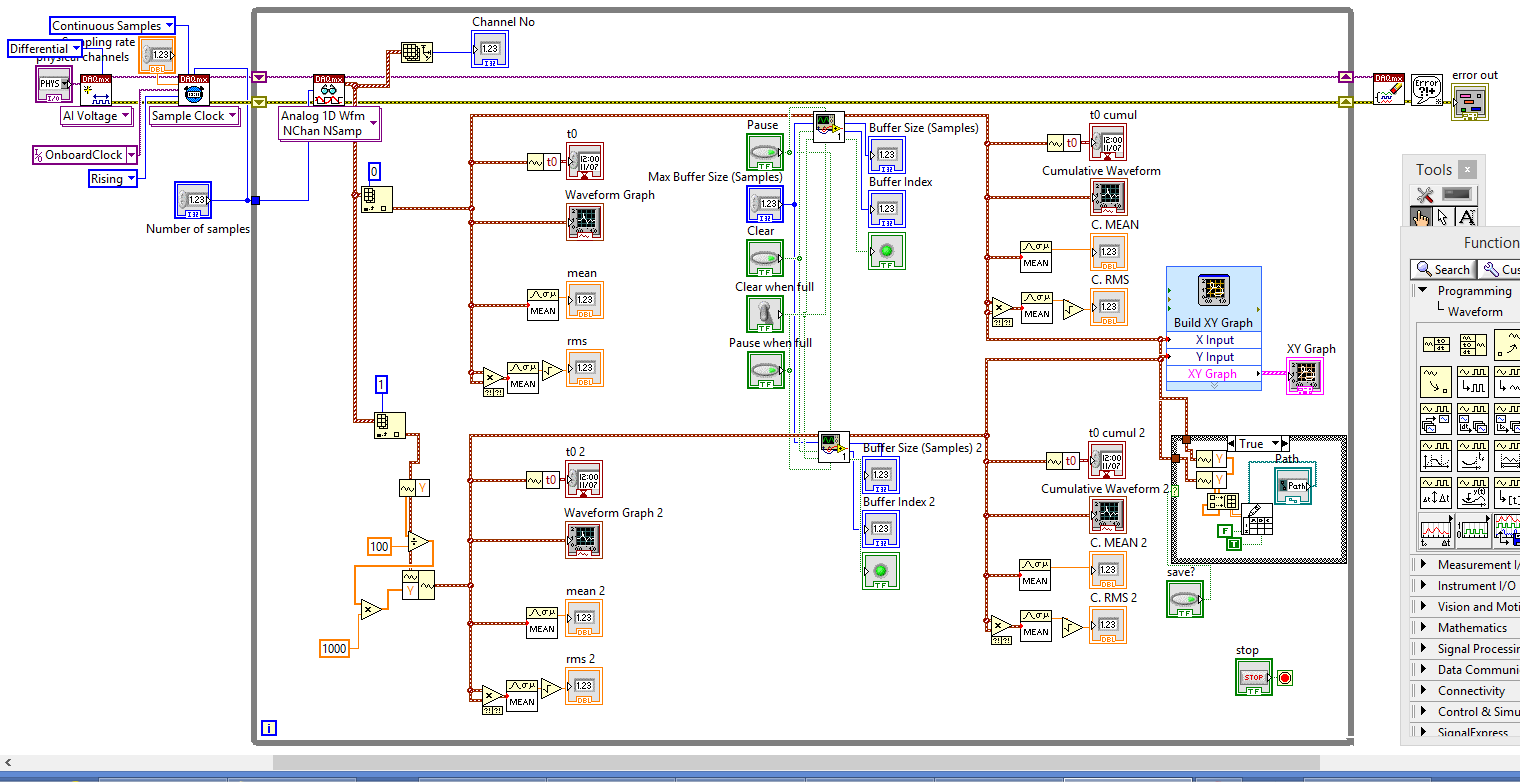
\includegraphics[width=\linewidth/1]{act1bp}
  \caption{The block diagram of the VI.}
  \label{fig:act1bp}
 \end{center}
\end{figure}

\begin{figure}[H]
 \begin{center}
  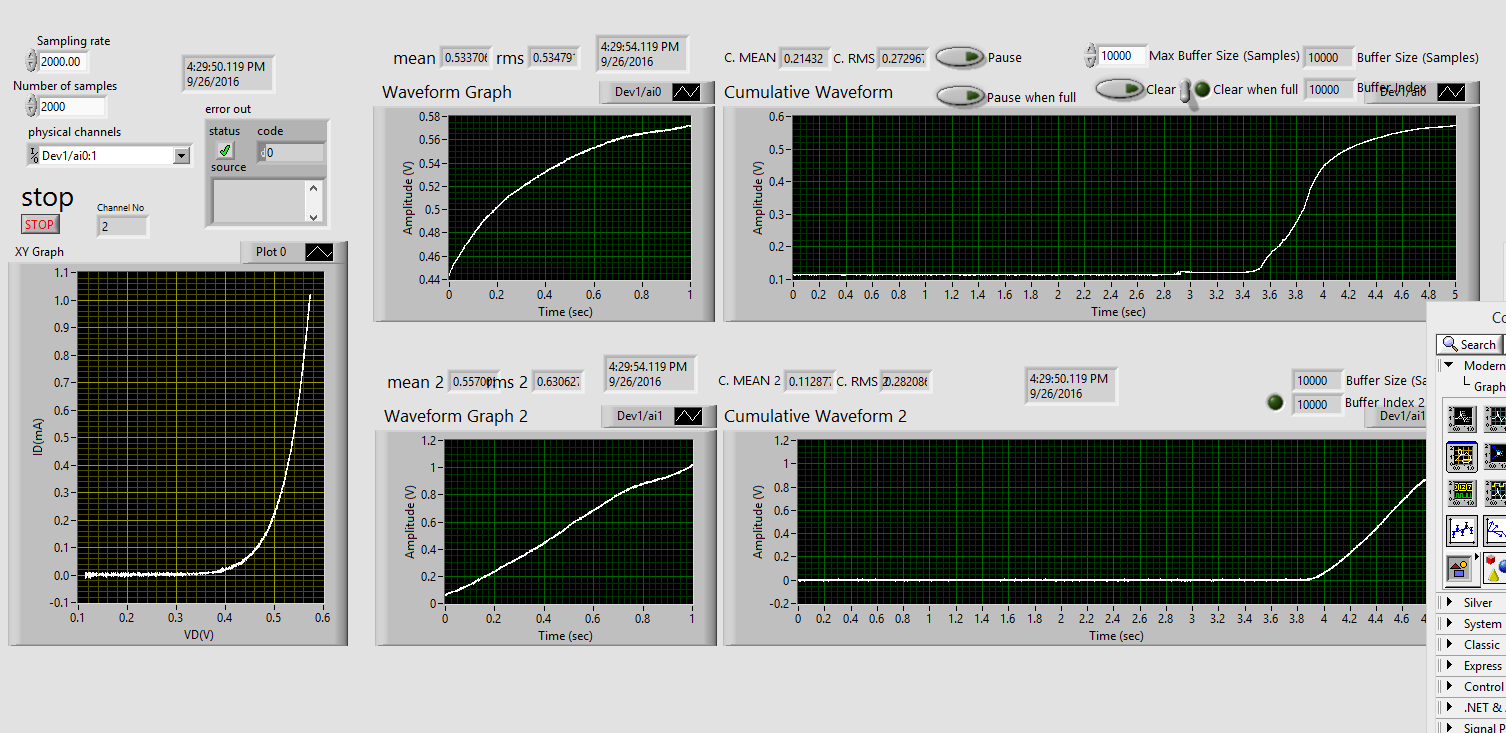
\includegraphics[width=\linewidth/1]{act1bias}
  \caption{The front panel image for forward bias IV measurements.}
  \label{fig:act1bias}
 \end{center}
\end{figure}

\begin{figure}[H]
 \begin{center}
  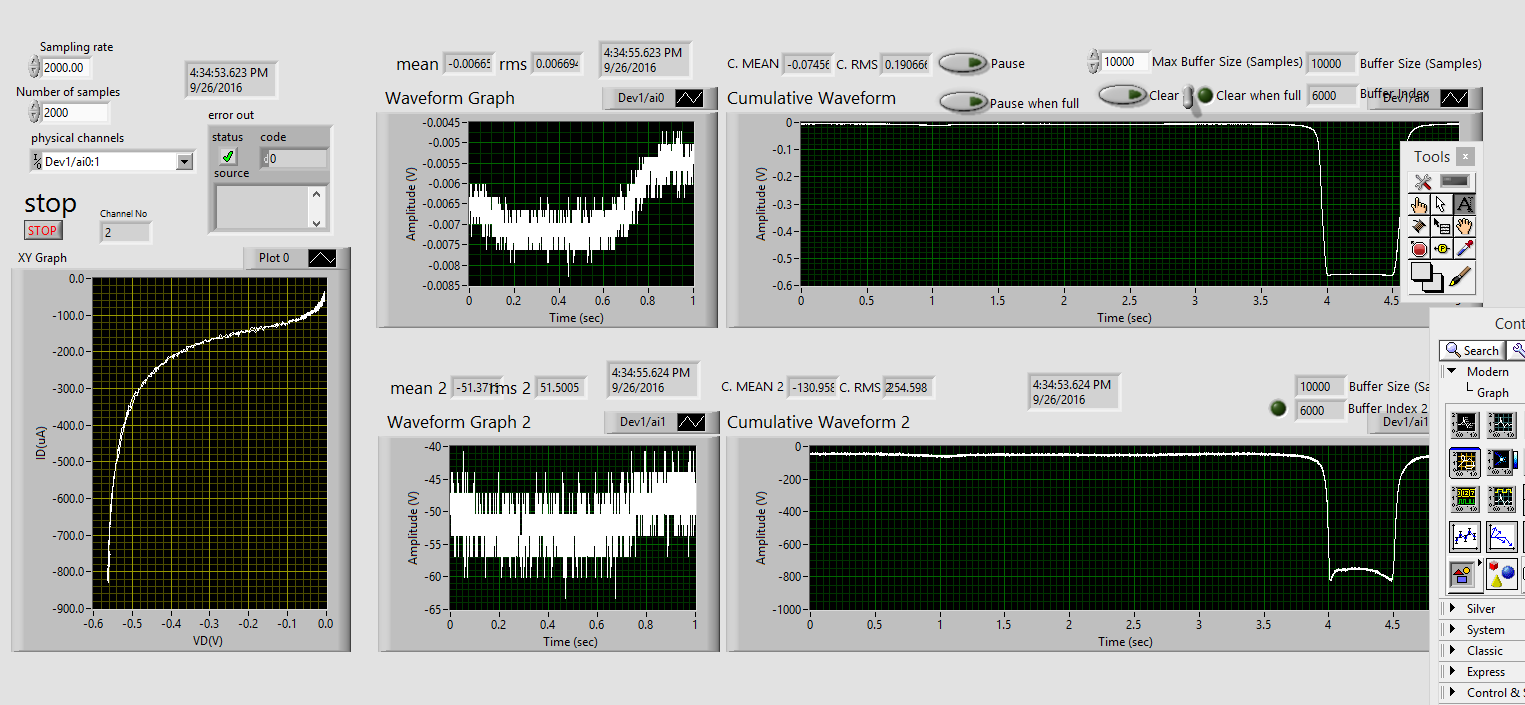
\includegraphics[width=\linewidth/1]{act1rev2}
  \caption{The front panel image for reverse bias IV measurements.}
  \label{fig:act1rev2}
 \end{center}
\end{figure}

$V_{\mathrm {s} }=5 V$

$V_{\mathrm {Dmax} }=0.58 V$

$I_{\mathrm {Dmax} }=1 mA$

$R_{\mathrm {3} }=100 \Omega$

$R_{\mathrm {2} }=470 \Omega$

$R_{\mathrm {1} }=4700 \Omega$

$\Rightarrow V_{\mathrm {R2} }=I_{\mathrm {Dmax} }*R_{\mathrm {3} }+V_{\mathrm {Dmax} }=0.1+0.58=0.68 V$

$\Rightarrow I_{\mathrm {R2} }={\frac {V_{\mathrm {R2} }}{R_{\mathrm {2} }}}=0.68/470=1.447 mA $

$\Rightarrow I_{\mathrm {total} }=I_{\mathrm {R2} }+I_{\mathrm {Dmax} }=1.447+1=2.447 mA $

$\Rightarrow P_{\mathrm {smax} }=I_{\mathrm {total} }*V_{\mathrm {s} }=0.002447*5=0.012 w $ \\[1em]

$ V_{\mathrm {R1} }=V_{\mathrm {s} }-V_{\mathrm {R2} }=5-0.68=4.32 V $

$\Rightarrow P_{\mathrm {R1} }=I_{\mathrm {total} }*V_{\mathrm {R1} }=0.002447*4.32=0.0106 w $ \\[1em]

$\Rightarrow P_{\mathrm {R2} }=I_{\mathrm {R2} }*V_{\mathrm {R2} }=0.001447*0.68=0.984 mw $ \\[1em]

$P_{\mathrm {R3} }=I_{\mathrm {D} }^2*R_{\mathrm {3} }=0.001^2*100=0.1 mw $

From the pictures, we can see that our knee voltage is around 0.45V, which is consistent with what we have read for the diode (0.7V$\sim{Silicon}$, 0.3V$\sim{Germanium}$). And the reverse saturation current is around 200 $\mu$ A, which we think is too large compared to what we expect.



\section{Activity II - Building a Circular Buffer VI for Continuous Analog Input Monitoring}


\begin{figure}[H]
 \begin{center}
  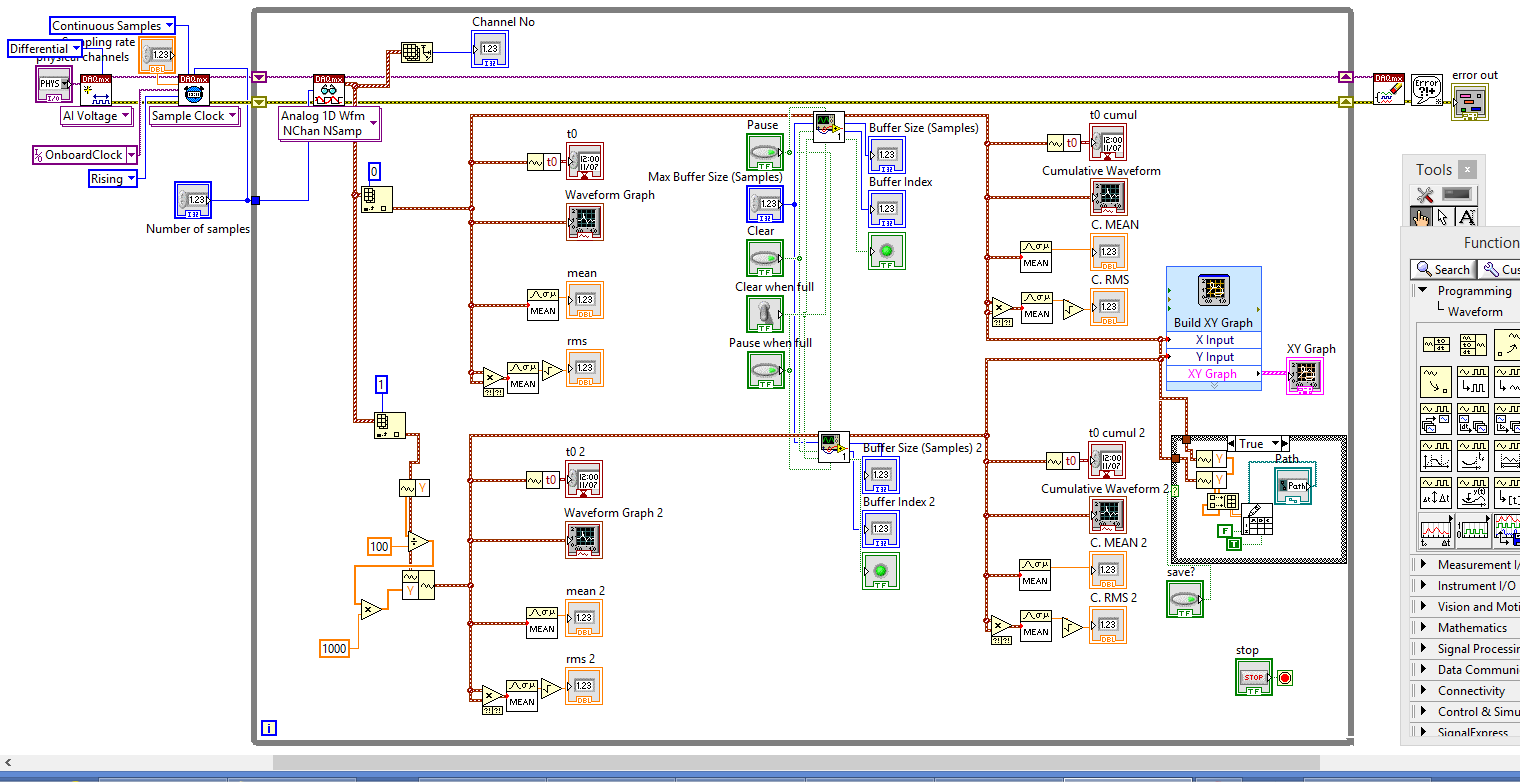
\includegraphics[width=\linewidth/2]{act1bp}
  \caption{The block diagram of the circular buffer VI for continuous analog input monitoring.}
  \label{fig:act1bp}
 \end{center}
\end{figure}

\begin{figure}[H]
 \begin{center}
  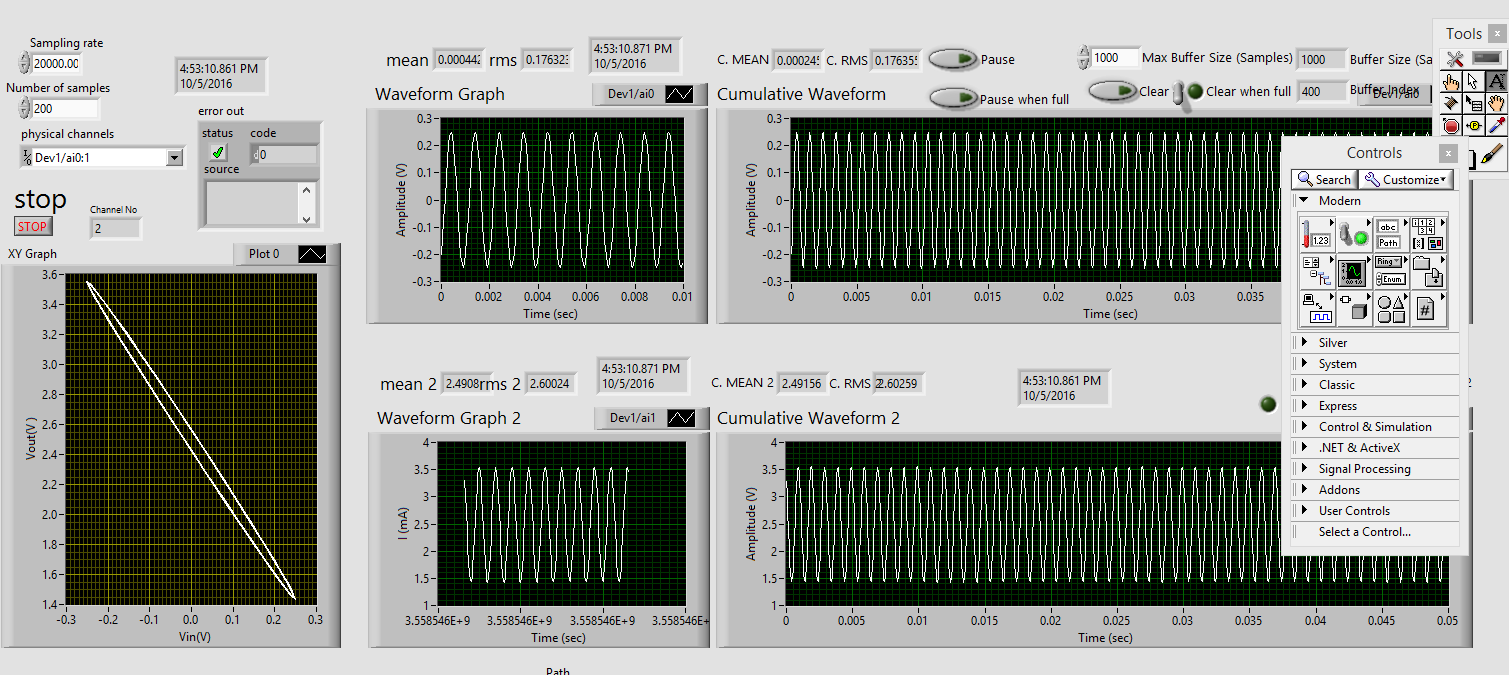
\includegraphics[width=\linewidth/2]{act2}
  \caption{The front panel of the circular buffer VI for continuous analog input monitoring.}
  \label{fig:act2}
 \end{center}
\end{figure}

And we saved the data file as genericDAQ_DataFile

\section{Activity III - Monitoring a Thermistor Using Your Circular Buffer VI and a Voltage Divider Circuit}

The relationship between {\displaystyle V_{\mathrm {Th} }, {\displaystyle R_{\mathrm {Th} }, {\displaystyle R_{\mathrm {1}\ } {\mathrm {and}\ }   {\displaystyle V_{\mathrm {1} } :


{\displaystyle V_{\mathrm {Th} }={\frac {R_{Th}}{R_{Th}+R_{1}}}\cdot V_{\mathrm {1} }} 

\Rightarrow  {\displaystyle R_{\mathrm {Th} }={\frac {V_{Th}}{V_{1}-V_{Th}}}\cdot R_{\mathrm {1} }} 

{V_{\mathrm {1} }=2.5 V}

{R_{\mathrm {1} }=10\ K\Omega}

\Rightarrow  {\displaystyle R_{\mathrm {Th} }={\frac {V_{Th}}{2.5-V_{Th}}}\cdot 10000}  

\

\begin{figure}[H]
 \begin{center}
  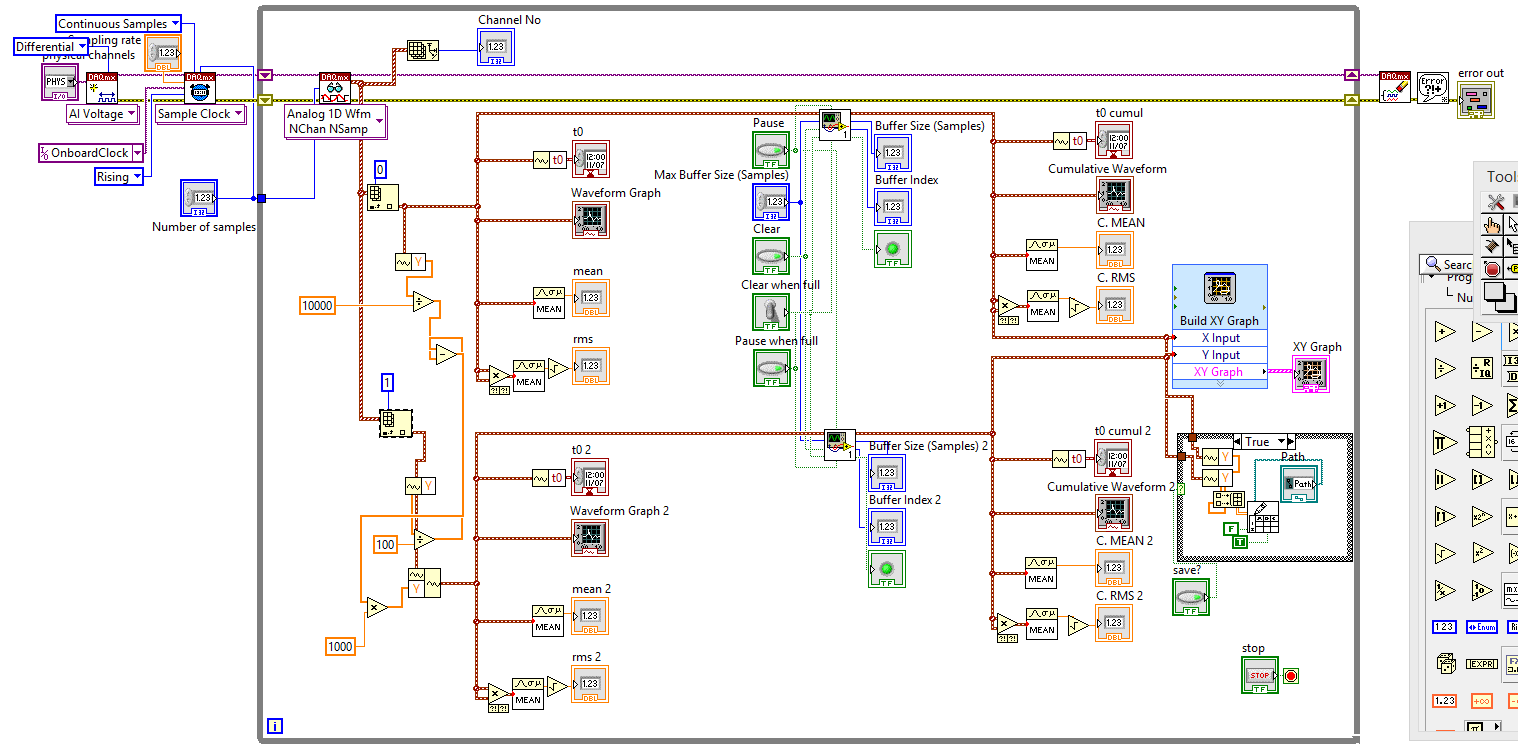
\includegraphics[width=\linewidth/2]{act3bp}
  \caption{The block diagram of the the modified circular buffer VI .}
  \label{fig:act3bp}
 \end{center}
\end{figure}

\begin{figure}[H]
 \begin{center}
  \includegraphics[width=\linewidth/2]{act3room}
  \caption{The front panel of the the modified circular buffer VI with room temperature.}
  \label{fig:act3room}
 \end{center}
\end{figure}

\begin{figure}[H]
 \begin{center}
  \includegraphics[width=\linewidth/2]{act3finger}
  \caption{The front panel of the the modified circular buffer VI with finger temperature.}
  \label{fig:act3finger}
 \end{center}
\end{figure}

As is seen from the pictures, the room temperature is about 25 $^{\circ}$C, which make sense. Then when we heated up the thermistor with our fingers, we could see the temperature increased and finally stopped at about 32.5 $^{\circ}$C. And if we remove our fingers, the temperature goes down and noise exists as the following picture shows.

\begin{figure}[H]
 \begin{center}
  \includegraphics[width=\linewidth/2]{act3noise}
  \caption{The front panel of the the modified circular buffer VI with noise.}
  \label{fig:act3noise}
 \end{center}
\end{figure}

\section{Activity IV - Monitoring a Thermistor Using Your Circular Buffer VI and a Wheatstone Bridge Circuit}

The following shows that when {\displaystyle V_{\mathrm {G}}=0} , {\mathrm {which\ is at\ the\ point\ of\ balance,\ the\ ratio\ of\ }} 

{\displaystyle {\begin{aligned}{\frac {R_{2}}{R_{1}}}&={\frac {R_{x}}{R_{3}}}\\[4pt]\Rightarrow R_{x}&={\frac {R_{2}}{R_{1}}}\cdot R_{3}\end{aligned}}} :

\begin{figure}[H]
 \begin{center}
  \includegraphics[width=\linewidth/2]{bridge}
  \caption{Wheatstone bridge.}
  \label{fig:bridge}
 \end{center}
\end{figure}

 Kirchhoff's first rule \Rightarrow
 
 {\displaystyle {\begin{aligned}I_{3}-I_{x}+I_{G}&=0\\
 
 I_{1}-I_{2}-I_{G}&=0\end{aligned}}} 
 
 Kirchhoff's second rule \Rightarrow
 
 {\displaystyle {\begin{aligned}(I_{3}\cdot R_{3})-(I_{G}\cdot R_{G})-(I_{1}\cdot R_{1})&=0\\
 
 (I_{x}\cdot R_{x})-(I_{2}\cdot R_{2})+(I_{G}\cdot R_{G})&=0\end{aligned}}}
 
 {\displaystyle I_{\mathrm {G}}=0} \Rightarrow
 
 {\displaystyle {\begin{aligned}I_{3}\cdot R_{3}&=I_{1}\cdot R_{1}\\
 
 I_{x}\cdot R_{x}&=I_{2}\cdot R_{2}\end{aligned}}} 
 
 \Rightarrow {\displaystyle R_{x}={{R_{2}\cdot I_{2}\cdot I_{3}\cdot R_{3}} \over {R_{1}\cdot I_{1}\cdot I_{x}}}} 
 
 \because {\displaystyle I_{\mathrm {3}}=I_{\mathrm {x}}},\ {\displaystyle I_{\mathrm {1}}=I_{\mathrm {2}}}
 
 \therefore {\displaystyle {\begin{aligned}{\frac {R_{2}}{R_{1}}}&={\frac {R_{x}}{R_{3}}}\\[4pt]\Rightarrow R_{x}&={\frac {R_{2}}{R_{1}}}\cdot R_{3}\end{aligned}}} ~\\

 And the following equation can also be derived:
 
 {\displaystyle V_{G}=\left({R_{2} \over {R_{1}+R_{2}}}-{R_{x} \over {R_{x}+R_{3}}}\right)V} \\[2em]

 In this lab:~\\
 
 \begin{figure}[H]
 \begin{center}
  \includegraphics[width=\linewidth/2]{act4bridge}
  \caption{activity 4: Wheatstone bridge.}
  \label{fig:act4bridge}
 \end{center}
 \end{figure}
 

 {\displaystyle V_{o}=\left({R_{1} \over {R_{4}+R_{1}}}-{R_{2} \over {R_{2}+R_{3}}}\right)V_{B}} 
 
 \Rightarrow {\displaystyle V_{o}=\left({R \over {R+R}}-{R+\Delta R \over {R+\Delta R+R}}\right)V_{B}=\left({1 \over {2}}-(1-{R \over {2R+\Delta R}})\right)V_{B}=\left({-{1 \over {2}}}+{{1 \over {2}}({1 \over {1+{\Delta R \over {2R}}}})\right)V_{B}} 
 
 We know that when x\textless\textless 1, (1+x)^\alpha \approx 1+\alpha x,\ {\mathrm {to\ lowest\ order\ in\ x}}
 
 So {\displaystyle \left(1+{\Delta R \over {2R}}\right)^{-1}} \approx {\displaystyle 1-{\Delta R \over {2R}}}
 
 \Rightarrow {\displaystyle V_{o} \approx \left({-{1 \over {2}}}+{{1 \over {2}}(1-{\Delta R \over {2R}}}})\right)V_{B}=-{\Delta R \over {4R}}V_{B}} ,\ {\mathrm {to\ lowest\ order\ in\ \Delta R}}
 
 \begin{figure}[H]
 \begin{center}
  \includegraphics[width=\linewidth/2]{act4room}
  \caption{The front panel of the VI with room temperature.}
  \label{fig:act4room}
 \end{center}
 \end{figure}
 
 \begin{figure}[H]
 \begin{center}
  \includegraphics[width=\linewidth/2]{act4finger}
  \caption{The front panel of the VI with finger temperature.}
  \label{fig:act4finger}
 \end{center}
 \end{figure}
 
 \begin{figure}[H]
 \begin{center}
  \includegraphics[width=\linewidth/2]{act4noise}
  \caption{The front panel of the VI with noise.}
  \label{fig:act4noise}
 \end{center}
 \end{figure}

By using the way of Wheatstone bridge circuit, which is, after we’ve achieved the null condition with the thermistor at ambient temperatures, we hooked up an amplifier to measure Vo. As seen from the pictures, this gives us much greater voltage resolution and hence a much greater temperature resolution. Our noise of the temperature showed that the resolution is around 0.06 $^{\circ}$C before, but it decreased to 0.005 $^{\circ}$C after. So the temperature change we think we could resolve for the present configuration is as small as 0.005 $^{\circ}$C.

\section{Addendum to Lab 4}

\begin{figure}[H]
 \begin{center}
  \includegraphics[width=\linewidth/2]{act4add}
  \caption{The front panel and the block diagram of the VI to plot the data from a previously saved text file.}
  \label{fig:act4add}
 \end{center}
 \end{figure}

The result is the same as what we got in the previous section.


\end{document}
